\fancyhead[LE]{\fontsize{8.5pt}{10pt}\selectfont\textbf{\textsf{\thepage}}\quad \textbf{\textsf{CHƯƠNG 1}}\quad \textsf{Các hàm số và Mô hình}}
\fancyhead[RO]{\fontsize{8.5pt}{10pt}\selectfont\textsf{MỤC 1.2}\quad \textbf{\textsf{\thepage}}}

\noindent
\begin{minipage}[t]{0.265\textwidth}
    \fontsize{8pt}{10pt}\selectfont
    \vspace*{165pt}
    \begin{center}
        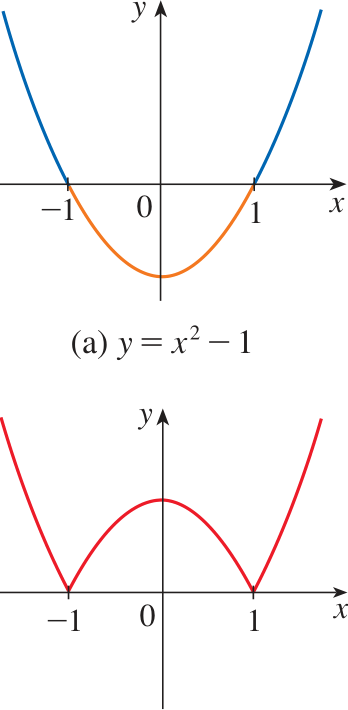
\includegraphics[width=0.92\linewidth]{images/p0075_fig10.png}
        \vspace{4pt}
        
        \textbf{\textsf{HÌNH 10}}
    \end{center}
\end{minipage}%
\hfill
\begin{minipage}[t]{0.708\textwidth}
    \fontsize{9.3pt}{13.2pt}\selectfont
    \textbf{\textsf{\color{stewartcyan}LỜI GIẢI}}\quad Nhận thấy rằng mỗi đường cong đều có dạng một đường hình sin bị tịnh tiến và co dãn. Quan sát đường màu xanh lam, ta thấy rằng ở vĩ độ của Philadelphia, thời gian ban ngày kéo dài khoảng $14{,}8$ giờ vào ngày 21 tháng 6 và $9{,}2$ giờ vào ngày 21 tháng 12, do đó biên độ của đường cong (hệ số mà ta cần dùng để dãn đường cong sin theo phương thẳng đứng) là $\frac{1}{2}(14{,}8 - 9{,}2) = 2{,}8$.

    Ta cần dãn đường cong sin theo phương ngang với hệ số là bao nhiêu nếu đo thời gian $t$ bằng ngày? Vì một năm có khoảng 365 ngày, chu kỳ của mô hình phải là 365. Nhưng chu kỳ của $y = \sin t$ là $2\pi$, vì vậy hệ số dãn theo phương ngang là $2\pi/365$.

    Ta cũng nhận thấy rằng đường cong bắt đầu một chu kỳ vào ngày 21 tháng 3, tức ngày thứ 80 trong năm, nên ta cần tịnh tiến đường cong sang phải 80 đơn vị. Ngoài ra, ta tịnh tiến đồ thị lên trên 12 đơn vị. Do đó, ta mô hình hóa độ dài thời gian ban ngày tại Philadelphia vào ngày thứ $t$ trong năm bằng hàm số
    \[
    L(t) = 12 + 2{,}8 \sin\left[ \frac{2\pi}{365}(t - 80) \right]
    \]
    \vspace{-1.2em}
    \hfill{\color{stewartcyan}$\blacksquare$}

    \vspace{0.8em}
    Một phép biến đổi khác cũng rất đáng quan tâm là lấy \textit{giá trị tuyệt đối} của một hàm số. Nếu $y = |f(x)|$, thì theo định nghĩa của giá trị tuyệt đối, $y = f(x)$ khi $f(x) \geqslant 0$ và $y = -f(x)$ khi $f(x) < 0$. Điều này cho ta biết cách suy ra đồ thị của $y = |f(x)|$ từ đồ thị của $y = f(x)$: phần đồ thị nằm phía trên trục $x$ được giữ nguyên, còn phần đồ thị nằm phía dưới trục $x$ được lấy đối xứng qua trục $x$.

    \vspace{0.8em}
    \noindent\textbf{\textsf{\color{stewartcyan}VÍ DỤ 5}}\quad Vẽ đồ thị của hàm số $y = |x^2 - 1|$.

    \vspace{0.3em}
    \noindent\textbf{\textsf{\color{stewartcyan}LỜI GIẢI}}\quad Trước tiên, ta vẽ parabol $y = x^2 - 1$ ở Hình 10(a) bằng cách tịnh tiến parabol $y = x^2$ xuống dưới 1 đơn vị. Ta thấy rằng đồ thị nằm phía dưới trục $x$ khi $-1 < x < 1$, do đó ta lấy đối xứng phần đồ thị đó qua trục $x$ để nhận được đồ thị của hàm số $y = |x^2 - 1|$ ở Hình 10(b).\hfill{\color{stewartcyan}$\blacksquare$}

    \vspace{1em}
    \noindent{\color{stewartcyan}\rule{1.2ex}{1.2ex}}\hspace{0.5em}\textbf{\textsf{\large Các phép toán kết hợp hàm số}}

    \vspace{0.4em}
    Hai hàm số $f$ và $g$ có thể được kết hợp để tạo thành các hàm số mới $f + g$, $f - g$, $fg$, và $f/g$ theo cách tương tự như cách chúng ta cộng, trừ, nhân, và chia các số thực.

    \vspace{0.6em}
    \begin{definitionbox}
        \textbf{\textsf{\color{stewartred}Định nghĩa}}\quad Cho hai hàm số $f$ và $g$, các hàm số \textbf{tổng}, \textbf{hiệu}, \textbf{tích}, và \textbf{thương} được định nghĩa bởi
        \begin{align*}
        (f + g)(x) &= f(x) + g(x) & (f - g)(x) &= f(x) - g(x) \\[4pt]
        (fg)(x) &= f(x)\,g(x) & \left(\frac{f}{g}\right)(x) &= \frac{f(x)}{g(x)}
        \end{align*}
    \end{definitionbox}

    \vspace{0.6em}
    Nếu miền xác định của $f$ là $A$ và miền xác định của $g$ là $B$, thì miền xác định của $f + g$ (và miền xác định của $f - g$) là giao $A \cap B$ vì cả $f(x)$ và $g(x)$ đều phải xác định. Chẳng hạn, miền xác định của $f(x) = \sqrt{x}$ là $A = [0, \infty)$ và miền xác định của $g(x) = \sqrt{2 - x}$ là $B = (-\infty, 2]$, do đó miền xác định của $(f + g)(x) = \sqrt{x} + \sqrt{2 - x}$ là $A \cap B = [0, 2]$.

    Miền xác định của $fg$ cũng là $A \cap B$. Do không thể chia cho 0, miền xác định của $f/g$ là $\{x \in A \cap B \mid g(x) \neq 0\}$. Ví dụ, nếu $f(x) = x^2$ và $g(x) = x - 1$, thì miền xác định của hàm phân thức $(f/g)(x) = x^2/(x - 1)$ là $\{x \mid x \neq 1\}$, hay $(-\infty, 1) \cup (1, \infty)$.

    Còn có một cách khác để kết hợp hai hàm số nhằm tạo ra một hàm số mới. Chẳng hạn, giả sử rằng $y = f(u) = \sqrt{u}$ và $u = g(x) = x^2 + 1$. Vì $y$ là một hàm số
\end{minipage}